\documentclass[bsc,logo,frontabs,twoside,singlespacing,normalheadings,parskip]{infthesis}\usepackage[]{graphicx}\usepackage[]{color}
%% maxwidth is the original width if it is less than linewidth
%% otherwise use linewidth (to make sure the graphics do not exceed the margin)
\makeatletter
\def\maxwidth{ %
  \ifdim\Gin@nat@width>\linewidth
    \linewidth
  \else
    \Gin@nat@width
  \fi
}
\makeatother

\definecolor{fgcolor}{rgb}{0.345, 0.345, 0.345}
\newcommand{\hlnum}[1]{\textcolor[rgb]{0.686,0.059,0.569}{#1}}%
\newcommand{\hlstr}[1]{\textcolor[rgb]{0.192,0.494,0.8}{#1}}%
\newcommand{\hlcom}[1]{\textcolor[rgb]{0.678,0.584,0.686}{\textit{#1}}}%
\newcommand{\hlopt}[1]{\textcolor[rgb]{0,0,0}{#1}}%
\newcommand{\hlstd}[1]{\textcolor[rgb]{0.345,0.345,0.345}{#1}}%
\newcommand{\hlkwa}[1]{\textcolor[rgb]{0.161,0.373,0.58}{\textbf{#1}}}%
\newcommand{\hlkwb}[1]{\textcolor[rgb]{0.69,0.353,0.396}{#1}}%
\newcommand{\hlkwc}[1]{\textcolor[rgb]{0.333,0.667,0.333}{#1}}%
\newcommand{\hlkwd}[1]{\textcolor[rgb]{0.737,0.353,0.396}{\textbf{#1}}}%

\usepackage{framed}
\makeatletter
\newenvironment{kframe}{%
 \def\at@end@of@kframe{}%
 \ifinner\ifhmode%
  \def\at@end@of@kframe{\end{minipage}}%
  \begin{minipage}{\columnwidth}%
 \fi\fi%
 \def\FrameCommand##1{\hskip\@totalleftmargin \hskip-\fboxsep
 \colorbox{shadecolor}{##1}\hskip-\fboxsep
     % There is no \\@totalrightmargin, so:
     \hskip-\linewidth \hskip-\@totalleftmargin \hskip\columnwidth}%
 \MakeFramed {\advance\hsize-\width
   \@totalleftmargin\z@ \linewidth\hsize
   \@setminipage}}%
 {\par\unskip\endMakeFramed%
 \at@end@of@kframe}
\makeatother

\definecolor{shadecolor}{rgb}{.97, .97, .97}
\definecolor{messagecolor}{rgb}{0, 0, 0}
\definecolor{warningcolor}{rgb}{1, 0, 1}
\definecolor{errorcolor}{rgb}{1, 0, 0}
\newenvironment{knitrout}{}{} % an empty environment to be redefined in TeX

\usepackage{alltt}     
\usepackage[page]{appendix}

\usepackage{chngpage}

\usepackage{amsmath}

\usepackage{pifont}
\newcommand{\cmark}{\ding{51}}\newcommand{\xmark}{\ding{55}}
\usepackage[
 backend=bibtex,
 natbib=true,
 style=ieee,
]{biblatex}
\addbibresource{report.bib}

\usepackage{fontspec}
\setmainfont[Mapping=tex-text,Numbers=OldStyle]{fbb}
\setsansfont[BoldFont="GillSans-SemiBold",Mapping=tex-text,Numbers=OldStyle,Scale=MatchLowercase]{Gill Sans}
\setmonofont[Mapping=tex-text,Scale=MatchLowercase]{Inconsolata}

\usepackage{booktabs}

\let\oldtabular\tabular
\renewcommand{\tabular}{\sffamily\oldtabular}

\renewcommand{\arraystretch}{1.3}

\usepackage[draft,bordercolor=white,backgroundcolor=yellow!60,linecolor=black,colorinlistoftodos]{todonotes}

\let\Oldtodo\todo
\renewcommand{\todo}[1]{\Oldtodo[inline]{#1}}

\usepackage{minted}

\renewcommand{\listoflistingscaption}{List of Listings}

\usepackage{subcaption}


\usepackage[]{hyperref}
\hypersetup{
    pdftitle={Storm on Multi-core},
    pdfauthor={Mark Nemec},
            bookmarksnumbered=true,
    bookmarksopen=true,
    bookmarksopenlevel=1,
        pdfstartview=Fit,
    pdfpagemode=UseOutlines,
    pdfpagelayout=TwoPageRight
}
\IfFileExists{upquote.sty}{\usepackage{upquote}}{}
\begin{document}

\title{Storm on Multi-core}
\author{Mark Nemec}
\course{Computer Science}
\project{4th Year Project Report}
\date{\today}

\abstract{
In recent years there has been a growing usage of data stream processing systems. However, data stream processing has been a province of distributed systems such as Apache Storm. This is because clusters offer better scale-out properties.

On the other hand, chip makers have been able to pack more and more transistors into a single processor chip. This resulted in a steady increase of the number of cores used in a single processor chip. It is possible that scale-out processors with high number of processor cores will be used for future throughput-based applications.

In this report we present Storm-MC, an API-compatible port of Apache Storm for multi-core. This system combines an easy to use API with implementation tailored to multi-core environments. This allows us to take existing applications written with Storm in mind and run them efficiently on a single server.

We show that running applications on Storm-MC can provide substantial improvement in throughput (up to 3.3x) compared to running them on Apache Storm in local mode.
}

\maketitle

\section*{Acknowledgements}
I would like to thank my supervisor, Dr. Stratis Viglas, for providing guidance every step of the way.

Furthermore, I would like to thank Daniela Kellerova who made sure I do not go insane while working on this project.

Finally, I would like to thank my parents who supported my studies at the University of Edinburgh. Without them this project would not be possible.

\pagenumbering{Roman}

\tableofcontents
\listoffigures
\listoftables
\listoflistings



\cleardoublepage
\pagenumbering{arabic}

\clearpage{}\chapter{Introduction}

\section{Motivation}

In recent years, there has been an explosion of cloud computing software. After Google published their paper on MapReduce \citep{dean2010mapreduce}, many new open-source frameworks for distributed computation have emerged, most notably Apache Hadoop \citep{ApacheHadoop} for batch processing and Apache Storm \citep{ApacheStorm} for real-time data stream processing.

These frameworks split the work that needs to be carried out and distribute it across nodes of a cluster. Commercial companies and researchers have been able to utilise these frameworks and create distributed systems which can accomplish things that would not be otherwise possible. This has mostly been allowed by the low price and good horizontal scaling properties of commodity hardware.


At the same time, chip makers have been increasing the number of cores in processors and now we are at a point where servers with 10-core processors are standard. Moreover, most high-end servers support multiple processor sockets thus furthering the parallelisation possible with a single machine even more.

The price of multi-core servers has been going down as well. In 2008, a typical Hadoop node had two dual-core processors and 4 GB of random access memory (RAM). Nowadays, a server with two eight-core processors and 256 GB of RAM can be purchased for roughly \$10,000 USD \citep{Kumar:2013:HSD:2536274.2536314}. Hence a single server today might have better processing power than a small cluster from a few years ago \citep{Kumar:2013:HSD:2536274.2536314}. If this trend continues there will be processors with even more cores in the near future.

Moreover, tiled processors have emerged as competitors to traditional processors in throughput-based computations \cite{Tilera}. These processors use a large number of tiles connected by an on-chip network and even though the single-thread performance of each tile is lower than the performance of a conventional core, the increased parallelism yields higher per-server throughput \cite{DBLP:conf/isca/Lotfi-KamranGFVKPAJIOF12}.

It is generally believed that writing parallel software is hard. The traditional techniques of message passing and shared memory require the programmer to manage the concurrency at a fairly low level. Apache Storm has become the de facto tool used in stream processing on a cluster and according to their ``Powered By" page there are tens of companies already using Storm to process their real-time data streams \cite{PoweredBy}. We believe there is a place for a real-time data stream processing system on multi-core and Storm's popularity and simple application programming interface (API) makes it the ideal candidate for porting.

\section{Main Idea}

The main idea of this report is to take the existing Apache Storm project and port it to multi-core. This is implemented in Storm-MC - a library with an API compatible with Apache Storm. Porting the Storm API allows programmers to take an existing application written with Apache Storm in mind and run it on a multi-core server. This way, we can avoid network latency and enjoy the significant performance improvements of a shared-memory environment.

\section{Project Contributions}

The primary contribution presented in this report is a port of Apache Storm that is tailored to multi-core environments.

\section{Structure of the Report}

The remainder of the report is structured as follows:

\begin{itemize}
	\item \textbf{Chapter 2} presents an overview of related literature and gives background on data stream processing and multi-core architectures.
	\item \textbf{Chapter 3} explains the concepts used in Apache Storm as well as the architecture of a Storm cluster.
	\item \textbf{Chapter 4} describes how Apache Storm was ported to multi-core and explains the design of Storm-MC.
	\item \textbf{Chapter 5} discusses the evaluation results of Storm-MC.
	\item \textbf{Chapter 6} presents conclusions of this report.
\end{itemize}
\clearpage{}

\clearpage{}\chapter{Literature Review}

The following chapter explains the concept of a data stream (\ref{sec:data_stream}), discusses advantages and disadvantages of multi-core (\ref{sec:multicore}), gives an overview of previous work on Apache Storm (\ref{sec:apache_storm}), and discusses other effort of porting distributed systems to multi-core (\ref{sec:similar_efforts}).

\section{Data Stream}
\label{sec:data_stream}

\textcite{golab2003issues} define data stream as as ``a real-time, continuous, ordered (implicitly by arrival time or explicitly by timestamp) sequence of items. It is impossible to control the order in which items arrive, nor is it feasible to locally store a stream in its entirety."

\subsection{Comparison to a Database Management System}

Historically, data has been stored into database management systems (DBMS) where it was later analysed the assumption being that there would be enough disk space to contain the data. This approach fits many purposes but real-time applications have recently started feeling the need to analyse rapidly changing data on-the-fly.

This has brought on an advent of data stream processing. Several stream-processing frameworks have emerged such as Apache Storm \citep{ApacheStorm}, Apache Spark \citep{ApacheSpark}, and Yahoo S4 \citep{YahooS4}. These frameworks, usually ran on a cluster, provide the user with abstractions which greatly simplify writing a real-time data stream processing application.

Whereas DBMSs excel at getting an exact answer to a query, data streams usually provide an approximate answer. The answer is approximate because it is usually correct only within a certain window of time, the query is simplified because it can only be ran in one pass, or because it is used with a sampling rate which does not include all events. A typical data stream analysis using windows and sampling is shown in Figure \ref{fig:stream}.

\subsection{Querying a Data Stream}

The assumption behind using a time window is that users of the real-time system are most likely interested in the most recent events. Sampling, on the other hand, is used to reduce the number of events used for a query \citep{Gaber:2005:MDS:1083784.1083789}.

\begin{figure}[!htb]
	\centering
	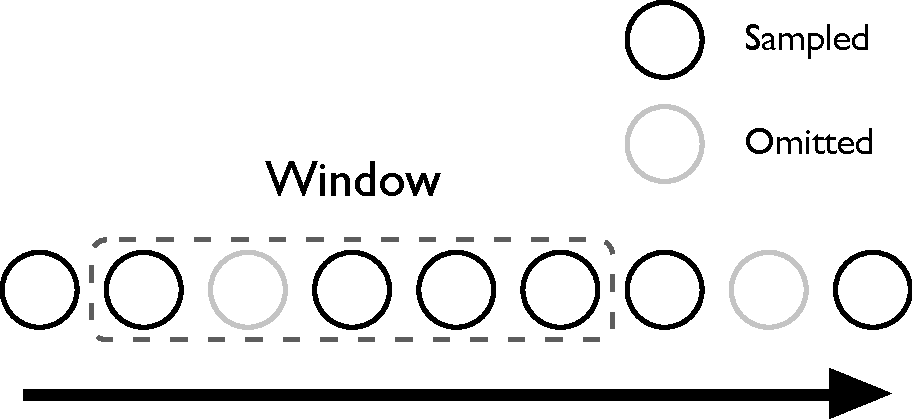
\includegraphics[scale=0.5]{pdf/stream.pdf}
	\caption{Stream Querying.}
	\label{fig:stream}
\end{figure}

Even though the answer might only be approximate it can have great value because the query is answered at the right time. Furthermore, even though the query may run only on a subset of data it is still possible to detect trends or system failures. For example, Twitter are using Apache Storm to run real-time analysis on millions of events per second for their analytics product Answers \citep{Solovey}.

In research, several techniques have been developed to enable real-time data stream mining. For example, the MOA environment created by \citet{Bifet:2010:MMO:1756006.1859903} enables running online machine learning methods using the WEKA machine learning workbench \citep{Holmes1994}.

\section{Multi-core}
\label{sec:multicore}

\textcite{akhter2006multi} define multi-core processor as a processor that has two or more independent execution cores. This means that every thread has a hardware execution environment entirely to itself which enables threads to run in a truly parallel manner.

Running an application on multi-core can in the best case produce a speedup equivalent to the number of cores. The best case is when an application is embarrassingly parallel i.e. there is no inter-thread communication. Even though data stream processing is not an embarrassingly parallel problem, running a producer-consumer application on multiple cores can produce significant speedup as shown in  \citep{Prat-Perez:2013:PPM:2450027.2450037}.

\subsection{Advantages Over Clusters}
\label{subsec:advantages}

There are several reasons why someone might prefer to deploy their data stream application to a single multi-core machine over a cluster:

\begin{description}
	\item[Communication Overhead] \hfill \\
	The latency of over-the-network communication is significantly higher than of two cores communicating on a single machine.
	\item[Lower Cost than a Data Centre] \hfill \\
	To run a distributed system on a cluster one would usually need to own a data centre. This comes with a high capital cost and increased maintenance costs than owning a single server.
	\item[More Control than with a Cloud Provider] \hfill \\
	Alternatively, one could rent out nodes on cloud computing services such as Amazon EC2 or Rackspace. While the cost of such services is acceptable the user does not have full control over their system.
\end{description}

\subsection{Disadvantages Over Clusters}
\label{subsec:disadvantages}

On the other hand, there are certain disadvantages in running a computation on a single multi-core machine rather than a cluster:

\begin{description}
	\item[Horizontal Scaling] \hfill \\
	Commodity hardware clusters offer better horizontal scaling than a single multicore server. If one needs to add nodes to the cluster it is as easy as purchasing more commodity hardware. On a multi-core machine it is not that simple. For example, a top of the line Intel\textsuperscript{\textregistered} Xeon\textsuperscript{\textregistered} Processor E5-2699 has support for 36 threads. Beyond that one would need to add another socket which essentially doubles the price. Moreover, the server would need to support multiple processor sockets.
	\item[Higher Short-term Cost than with a Cloud Provider] \hfill \\
	In short-term the cost of purchasing a server may be significantly higher than renting out a cluster from a cloud computing service. Thus, it makes most sense to run an application on multi-core as a medium- to long-term investment.
	\item[More Maintenance than with a Cloud Provider] \hfill \\
	Owning a server requires more maintenance than simply renting it out from a cloud provider. A cloud provider usually does  all the necessary maintenance and can provision a new machine very easily. Hence it is advantageous to use multi-core only if one can afford to maintain them as well.
\end{description}


\section{Apache Storm}
\label{sec:apache_storm}

Apache Storm is an open source distributed real-time computation system. Storm was Originally created by Nathan Marz while working at BackType. \cite{NathanAbout} BackType was later acquired by Twitter which is when Storm became open source. Storm was incubated into Apache with version 0.9.1 and became a top-level Apache project in September 2014.

Storm was developed to run on top of a cluster where nodes execute components of a computation in parallel. Running Storm on a cluster of commodity hardware gives it good horizontal scaling properties. Running separate components in parallel allows the system to execute in real time.

\subsection{Dependencies}

Storm has five major dependencies:

\begin{description}
	\item[Apache Zookeeper] \hfill \\
	Apache Zookeeper \citep{ApacheZookeeper} is an open source server that allows reliable distributed coordination. Storm uses Apache Zookeeper to maintain state which is then read and written to by nodes of a Storm cluster. More detail on how Storm uses Zookeeper is given in section \ref{subsec:zookeeper}.
	\item[Apache Thrift] \hfill \\
	Apache Thrift \citep{ApacheThrift} is a cross-language framework for developing services. It allows you to write a definition file for services and data types required by your application and automatically generates interface code which supports remote procedure calls and serialisation of the data types.
	\item[Kryo] \hfill \\
	Kryo \citep{EsotericKryo} is a serialisation library. It is used by Storm to serialise objects when sent over the network between nodes of a cluster.
	\item[Netty] \hfill \\
	Netty \citep{Netty} is an asynchronous event-driven network application framework. Storm utilises Netty to send intra-cluster messages. Thus when a node produces a result to be consumed by another node of the cluster it sends a message over the network using the TCP protocol implemented in Netty.
	\item[LMAX Disruptor] \hfill \\
	LMAX Disruptor \cite{LMAXDisruptor} is a high-performance data structure used to exchange data between concurrent threads. It uses a lock-free implementation of a ring buffer which components of a Storm program running on the same node a cluster use to exchange messages.
\end{description}

\subsection{Usage of Apache Storm}

Storm works particularly well with sister Apache projects such as Apache Kafka \cite{ApacheKafka} and Apache HBase \cite{ApacheHBase}. Apache Kafka is a messaging broker that is often used as the missing link between producers and consumers of a cluster. Apache HBase is a big data-store that allows real-time random reads and writes modelled after Google's Bigtable project \cite{Chang:2008:BDS:1365815.1365816}.

Storm is reportedly used by 81 companies listed on their website \cite{PoweredBy} and many others. Storm's popularity is one of the reasons why it was chosen for this project. Furthermore, we believe that the concepts used in Storm (explained further in section \ref{sec:concepts}) apply to many different situations and many applications can be easily adapter to work on top of Storm.

There has been significant research in optimising computations running on Apache Storm. For example, \cite{Chatzistergiou:2014:FHN:2661829.2661882} looked at how to reconfigure a Storm job by reallocating component tasks to minimise communication cost. A domain specific language for defining Storm jobs was proposed in \cite{DBLP:conf/fedcsis/ChandrasekaranSA14}. Finally, \cite{dimsonhailstorm} ported Storm to Haskell and looked at how to provide exactly once semantics.

\section{Similar Efforts}
\label{sec:similar_efforts}

Currently data stream processing is a province of distributed systems such as the ones mentioned in the previous section. Most languages support parallel execution and there are many libraries that ease the process of writing parallel programs on a single multi-core machine. However, they are not tailored to data stream processing and usually require the programmer to do the heavy lifting rather than abstract it away.

There has been effort to port Hadoop to multi-core in \citep{Kumar:2013:HSD:2536274.2536314} (Hone) as well as port of Google's MapReduce in \citep{ranger2007evaluating} (Phoenix). However, to our knowledge there has not been effort to port Storm or any other distributed real-time data stream system to multi-core.

\section{Summary}

Distributed real-time computation systems such as Apache Storm provide programmers with abstractions that make it very easy to implement a data stream processing applications on top of  a cluster. However, in case of single multi-core machines there are not any obvious software choices. While several frameworks that allow the programmer to parallelise the computation exist, they are not really tailored to data stream processing.

The following chapters provide a closer analysis of Apache Storm as well as a port of Apache Storm for a single multi-core machine.
\clearpage{}

\clearpage{}\chapter{Background}

In this chapter we give background information necessary to understand the design of Storm-MC. We give a quick overview of Apache Storm (\ref{sec:storm_overview}), explain the concepts used in Storm (\ref{sec:concepts}), show an example Storm program (\ref{sec:example_topology}), give details about the underlying architecture of Storm (\ref{sec:storm_arch}), and finally describe the serialisation used by Storm (\ref{sec:serialisation}).

\section{Storm Overview}
\label{sec:storm_overview}

Apache Storm was developed in a mix of Java and Clojure. As mentioned by the author of Storm in \cite{Marz_2014}, writing the Storm interfaces in Java ensured large potential user-base while writing the implementation in Clojure increased productivity.

To ensure API compatibility with Storm, Storm-MC was developed using the same set of languages. This allowed for code reuse and not having to re-implement functionality already present in Storm. Hence, in the following sections we describe Storm in greater detail in hope that this will later clarify design choices made for Storm-MC.

\section{Storm Concepts}
\label{sec:concepts}

\subsection{Core Concepts}

There are several core concepts used by Storm and hence by extension Storm-MC as well. These concepts are put together to form a simple API that allows the programmer to break down a computation into separate components and define how these components interact with each other. The three core concepts of Storm are:

\begin{description}
  \item[Spout] \hfill \\
  A spout is a component that represents the source of a data-stream. Typically, a spout reads from a message broker such as RabbitMQ \cite{RabbitMQ} or Apache Kafka but can also generate its own stream or read from somewhere like the Twitter streaming API \citep{TwitterStreaming}.
  \item[Bolt] \hfill \\
  A bolt is a component that transforms tuples from its input data stream and emits them to its output data stream. A bolt can perform a range of functions e.g. filter out tuples based on some criteria or perform a join of two different input streams.
  \item[Topology] \hfill \\
  The programmer connects spouts and bolts in a directed graph called topology which describes how the components interact with each other. The topology is then submitted to Storm for execution.
\end{description}

\subsection{Additional Concepts}

\begin{description}
  \item[Stream] \hfill \\
  A stream is defined as an unbounded sequence of tuples. Streams can be thought of as edges of a topology connecting bolts and spouts (vertices).
  \item[Tuple] \hfill \\
  A tuple wraps named fields and their values. The values of the fields can be of different types. When a component emits a tuple to a stream it sends that tuple to every bolt subscribed to the stream.
  \item[Stream Grouping] \hfill \\
  Every bolt needs to have a type of stream grouping associated with it. This grouping decides the means of distributing the tuples coming from the bolt's input streams amongst the instances of the bolt task. Following are the possible types of stream grouping:
  \begin{description}
  	\item[Shuffle] Randomly partition the tuples among all the bolt tasks.
  	\item[Fields] Hash on a subset of the tuple fields. All tuples with same values of those fields will go to same bolt task.
  	\item[All] Replicate the entire stream to all the bolt tasks.
  	\item[Direct] The producer of the tuple decides which task of the bolt will receive this tuple.
  	\item[Global] Send the entire stream to a single bolt task.
  	\item[Local or Shuffle] Prefer sending to executors in the same worker process, if that is not possible use same strategy as Shuffle.
  \end{description}
\end{description}

Users are also able to specify their own custom grouping by implementing the \texttt{CustomStreamGrouping} interface.

All the components of a Storm topology execute in parallel. The user can specify how much parallelism he wants associated with every component and Storm spawns the necessary number of threads. This is done through a configuration file, defined in YAML, which is submitted along with the topology.

There are two additional bolts running for every topology:

\begin{description}
	\item[Acker] \hfill \\
	The Acker bolt guarantees fault tolerance for the topology. It tracks every tuple that was produced and ensures that the tuple has been acknowledged by every bolt of the stream.
	\item[System Bolt] \hfill \\
	The System bolt is useful in two ways:
	\begin{description}
		\item[Metrics] System bolt collects metrics on the local Java Virtual Machine (JVM). Other components can subscribe to these metrics and receive their values at  regular intervals.
		\item[Ticks] Components of a topology can subscribe to receive tick tuples in regular intervals. These tuples can be used to trigger some event of a component.
	\end{description}
\end{description}

\section{Example Topology}
\label{sec:example_topology}

\begin{figure}[!htb]
	\centering
	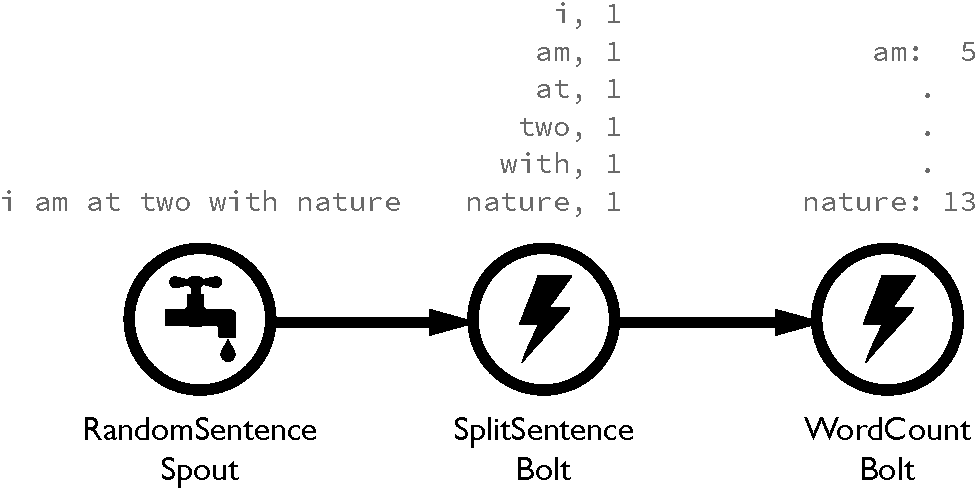
\includegraphics[scale=0.475]{pdf/wordcount_topology.pdf}
	\caption{WordCount topology.}
	\label{fig:wordcount_topology}
\end{figure}

A classic example used to explain Storm topologies is the WordCount topology. In this topology, there is a spout generating random sentences, a bolt splitting the sentences on white space, and a bolt counting occurrences of every word. Figure \ref{fig:wordcount_topology} shows how we could represent this topology graphically.

This may seem as a simplistic example but it is useful when demonstrating how easy it is to implement a working topology using the Storm API.

Listing \ref{listing:wordcount_topology} shows how the topology is put together in Storm to form a graph of components. Storm uses the Builder design pattern \citep{gamma1994design} to build up the topology which is then submitted to Storm for execution. The last argument to the \texttt{setBolt}/\texttt{setSpout} method is the number of parallel tasks we want Storm to execute for the respective component. For implementation of the spout and bolts used in this topology, refer to appendix \ref{ch:listings}.

\begin{listing}[!htb]
\inputminted{java}{code/WordCountTopology.java}
\caption{WordCountTopology.java}
\label{listing:wordcount_topology}
\end{listing}

\section{Storm Architecture}
\label{sec:storm_arch}

\begin{figure}[!htb]
	\centering
	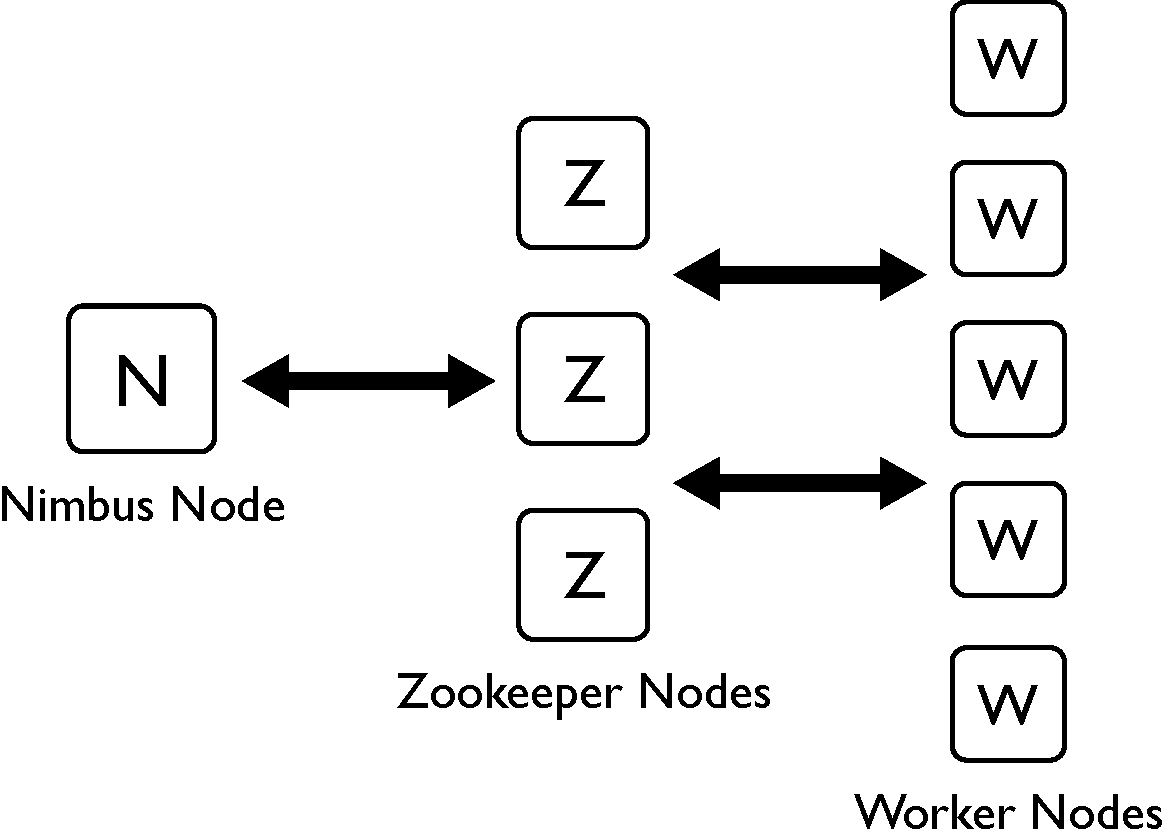
\includegraphics[scale=0.4]{pdf/storm_arch.pdf}
	\caption{Apache Storm Architecture.}
	\label{fig:storm_arch}
\end{figure}


A Storm cluster adopts the Master-Worker pattern. To set up a Storm topology, the user launches daemon processes on nodes of the cluster and submits the topology to the master node, also called Nimbus. The worker nodes receive task assignments from the master and execute the tasks assigned to them. The coordination between the master node and the worker nodes is handled by nodes running Apache Zookeeper. Figure \ref{fig:storm_arch} shows a graphical representation of Storm Architecture.

\subsection{Nimbus Node}

The master node runs a server daemon called Nimbus. The main role of Nimbus is to receive topology submissions from clients. Upon receiving a topology submission, Nimbus takes the following steps:

\begin{description}
	\item[Validate the topology] \hfill \\
	The topology is validated using a validator to ensure that the submitted topology is valid before trying to execute it. The user can use his own validator by implementing the \texttt{ITopologyValidator} interface or use the default validator provided by Storm.
	\item[Distribute the topology source code] \hfill \\
	Nimbus ensures that the workers involved in the topology computation have the source code by sending it to all nodes of the cluster.
	\item[Schedule the topology] \hfill \\
	Nimbus runs a scheduler that distributes the work among workers of the cluster. Similarly to validation, the user can use his own scheduler by implementing the \texttt{IScheduler} interface or use the default scheduler provided by Storm. The default scheduler uses a simple Round-robin strategy \citep{Aniello_Baldoni_Querzoni_2013}.
	\item[Activate the topology] \hfill \\
	Nimbus transitions the topology to active state which tells the worker nodes to start executing it.
	\item[Monitor the topology] \hfill \\
	Nimbus continues to monitor the topology by reading heartbeats sent by the worker nodes to ensure that the topology is executing as expected and worker nodes have not failed.
\end{description}


Nimbus is an Apache Thrift \cite{ApacheThrift} service (more on Thrift in section \ref{sec:serialisation}) that listens to commands submitted by clients and modifies the state of a cluster accordingly. Following are the commands supported by Nimbus:

\begin{description}
	\item[Submit a topology] \hfill \\
	Clients can submit a topology defined in a Java Archive (JAR) file. The Nimbus service then ensures that the topology configuration and resources are distributed across the cluster and starts executing the topology as previously described.
	\item[Kill a topology] \hfill \\
	Nimbus can stop running a topology and remove it from the cluster. The cluster can still continue executing other topologies.
	\item[Activate/deactivate a topology] \hfill \\
	Topologies can be deactivated and reactivated by Nimbus. This could be useful if the spout temporarily cannot produce a stream and the user does not want the cluster to execute idly.
	\item[Rebalance a topology] \hfill \\
	Nimbus can rebalance a topology across more nodes. Thus if the number of nodes in the cluster ever changes the user can increase or decrease the number of nodes involved in the topology computation.
\end{description}

\subsection{Worker Nodes}

The worker nodes run a daemon called Supervisor. There are 4 layers of abstraction which control the parallelism of a worker node.

\begin{description}
	\item[Supervisor] \hfill \\
	A supervisor is a daemon process the user runs on a worker node to make it part of the cluster. It launches worker processes and assigns them a port they can receive messages on. Furthermore, it monitors the worker processes and restarts them if they fail. A worker node runs only one supervisor process.
	\item[Worker] \hfill \\
	A worker process is assigned a port and listens to tuple messages on a socket associated with the port. A worker launches executor threads as required by the topology. Whenever it receives a tuple, it puts it on a receive queue of the target executor.
	
	Furthermore, the worker has a transfer queue where its executors enqueue tuples ready to be sent downstream. There can be multiple worker processes running inside one supervisor.
	\item[Executor] \hfill \\
	An executor controls the parallelism within a worker process. Every executor runs in a separate thread. An executor's job is to pick up tuples from its receive queue, perform the task of a component it represents, and put the transformed tuples on the transfer queue of the worker. There can be many executors running inside one worker and an executor performs one (the usual case) or more tasks.
	\item[Task] \hfill \\
	A task represents the actual tuple processing function. However, within an executor thread all the tasks are executed sequentially. The main reason for having tasks is that the number of tasks stays the same throughout the lifetime of a topology but the number of executors can change (by rebalancing). Thus if some worker nodes in the cluster go down, the topology can continue executing with the same number of tasks as before.
\end{description}

\subsection{Zookeeper Nodes}
\label{subsec:zookeeper}

The Storm cluster contains a number of Zookeeper nodes which coordinate the communication between Nimbus and the worker nodes. Storm does this by storing the state of the cluster on the Zookeper nodes where both Nimbus and worker nodes can access it.

The cluster state contains worker assignments, information about topologies, and heartbeats sent by the worker nodes to be read by Nimbus. Apart from the cluster state, Storm is completely stateless. Hence, if the master node or a worker node fail the cluster continues executing and the node will get restarted if possible. The only time the cluster stops executing  completely is if all the Zookeper nodes die.

\section{Serialisation}
\label{sec:serialisation}

Since Storm topologies execute on a cluster all components need to be serialisable. This is achieved with Apache Thrift. Components are defined as Thrift objects and Thrift generates all the Java serialisation code automatically.

Furthermore, since Nimbus is a Thrift service Thrift generates all the code required for remote procedure call (RPC) support. This allows defining topologies in any of the languages supported by Thrift and easy cross-language communication with the Nimbus service.
\clearpage{}

\clearpage{}\chapter{Bringing Storm to Multi-core}

The following chapter explains the design of Storm-MC. We describe how Apache Storm behaves in a multi-core environment (\ref{sec:storm_on_mc}), how the Storm architecture was ported over to multi-core (\ref{sec:storm_mc_arch}), how Storm-MC was implemented  (\ref{sec:implementation}), and we list feature differences between Apache Storm and Storm-MC (\ref{sec:differences}).

\section{Apache Storm on Multi-core}
\label{sec:storm_on_mc}

To begin, we discuss why Apache Storm does not perform optimally in a multi-core environment. Storm can be ran in local mode where it emulates execution on a cluster. This mode exists so that it is possible to debug and develop topologies without needing access to a cluster. However, there are several reasons why the local mode is not as performant as it could be.

\subsection{Tuple Processing Overhead}

\begin{figure}[!htb]
	\centering
	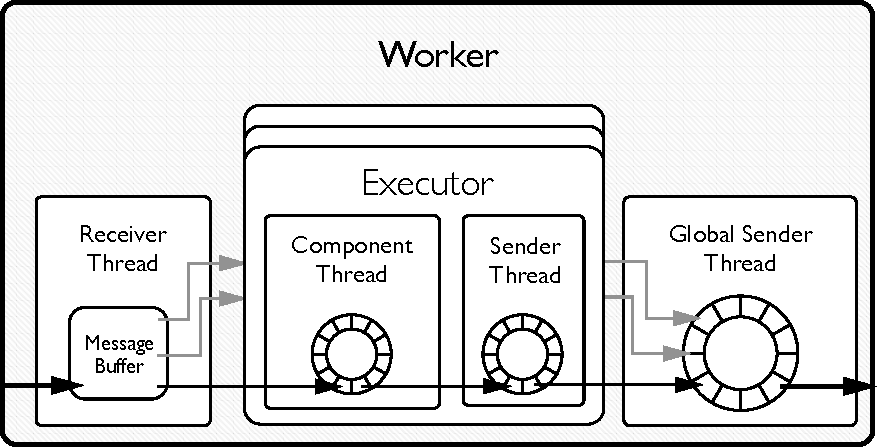
\includegraphics[scale=0.7]{pdf/worker_inside.pdf}
	\caption{Tuple processing in Apache Storm.}
	\label{fig:worker_inside}
\end{figure}

Figure \ref{fig:worker_inside} shows how tuple processing is implemented inside a Storm worker process. The tuple is read from a message buffer by the receiver thread of the worker and put on a receive queue of the target executor. The tuple is then picked up by the component thread of the executor for task execution.

After the component thread has executed the task it puts the tuple on the executor send queue. There, it is picked up by the executor sender thread which puts the tuple on the global send queue of the worker. Finally, the global sender thread of the worker serialises the tuple and sends it downstream.

Alternatively, if the tuple is forwarded to an executor in the same worker process it is put on the receive queue of the corresponding executor directly after task execution.

The queues used in Storm are implemented as ring buffers using the LMAX Disruptor library \citep{LMAXDisruptor}. Detailed background on how Disruptor works and its performance benchmarks can be found in \citep{Thompson_Farley_Barker_Gee_Stewart_2011}.

There is significant overhead required to simulate sending tuples to executors in other worker nodes. For one, there is the overhead from the tuple passing through the three queues of a worker. The authors of LMAX Disruptor showed that a three step pipeline has half the throughput of a single consumer-producer pipeline \citep{DisruptorWiki}.

Furthermore, to emulate over-the-network messages Storm uses a \texttt{Hashmap} of \texttt{LinkedBlockingQueue}s which according to \cite{Thompson_Farley_Barker_Gee_Stewart_2011} has several orders of magnitude lower performance than the Disruptor. Due to less write contention, lower concurrency overhead, and being more cache-friendly the Disruptor pattern can offer latency of inter-thread messages lower than 50 nanoseconds and a throughput of over 25 million messages per second \cite{Thompson_Farley_Barker_Gee_Stewart_2011}.

\subsection{Thread Overhead}

\begin{description}
	\item[Acker Bolt] \hfill \\
	The Acker bolt ensures that tuples propagate through a topology. In Storm it is included in every topology. It can be disabled via the configuration file in which case it is mostly idle since it does not receive any tuples. However, it can still use up resources especially if it waits fort tuples using a busy waiting strategy.
	\item[Heartbeats \& Timers] \hfill \\
	Every worker has a heartbeat thread that simulates sending heartbeat messages to the Nimbus node. It does this by writing to a local cache which is persisted to a file by a write on every heartbeat. Since the write is implemented using the \texttt{java.io} package the write is blocking - the thread cannot continue until the write is completed. While heartbeats are essential in cluster mode to signal the node being alive, there is no need for them in local mode.
	\item[Zookeeper Emulation] \hfill \\
	More overhead is produced by a local Zookeper server which emulates the Zookeeper nodes of a cluster. Running the Zookeeper server is a massive addition to the list of overheads as shown in the following paragraphs. The purpose of Zookeeper is to maintain states of running topologies and nodes of the cluster. As we will show in the following sections maintaining this state on multi-core is not necessary.
\end{description}

During profiling we found that a topology with one worker and three executors was being executed with 55 threads (not including system JVM threads and threads created by the profiler). Table \ref{table:breakdown} shows a breakdown of what the individual threads were used for.

\begin{table}[htb!]
\centering
\small
\begin{tabular}{@{}ll@{}}
    \textbf{Spout Parallelism} & \textbf{\# of Threads} \\ \toprule
    Main Thread & 1  \\
	Worker Sender \& Receiver Threads & 2  \\
    Acker \& System Component Threads & 2  \\
    Executor Component Threads & 3  \\
    Executor Sender Threads & 5  \\
    Various Timers \& Event Loops & 14  \\
    Zookeper Server & 28  \\
\end{tabular}
\caption{Threads used by Storm to execute a topology with three executors.}
\label{table:breakdown}
\end{table}

To find out what state the threads were actually in at any given time the topology was executed for three minutes and a JVM thread dump was recorded every second. The average results of this experiment can be observed in table \ref{table:dump} and the state distribution over time can be seen in Figure \ref{fig:dump-plot}.

\begin{table}[htb!]
\centering
\small
\begin{tabular}{@{}lc@{}}
    \textbf{Spout Parallelism} & \textbf{\# of Threads} \\ \toprule
    RUNNABLE & 8  \\
	TIMED WAITING & 22  \\
    WAITING & 25  \\
\end{tabular}
\caption{Average number of recorded thread states over a three minute period.}
\label{table:dump}
\end{table}

\begin{knitrout}
\definecolor{shadecolor}{rgb}{0.969, 0.969, 0.969}\color{fgcolor}\begin{figure}[!htb]
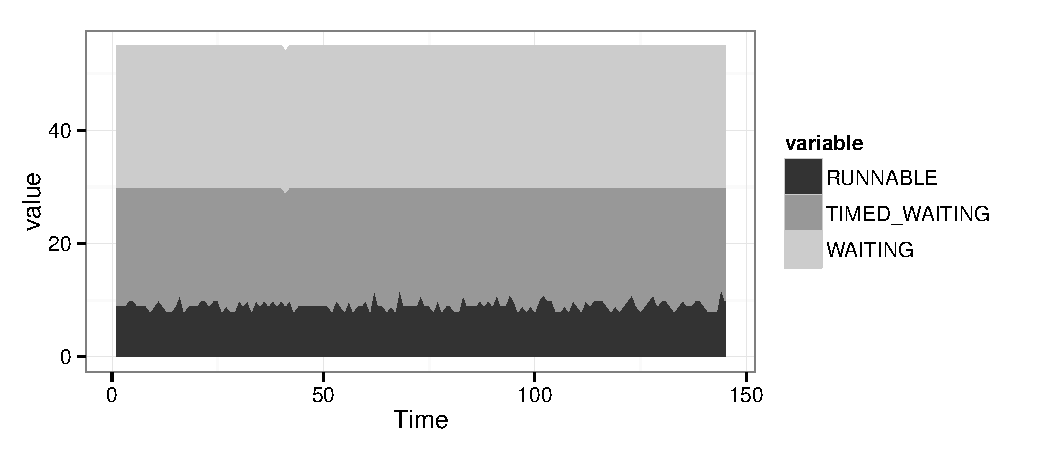
\includegraphics[width=\maxwidth]{figure/dump-plot-1} \caption[Thread state distribution over time]{Thread state distribution over time.}\label{fig:dump-plot}
\end{figure}


\end{knitrout}

Even though three minutes may seem to be a short amount of time the fact that there is almost no variation shows that it is sufficient. As can be seen from the table, most of the threads were either in state \texttt{WAITING} or \texttt{TIMED WAITING}. According to the Java documentation on thread states \citep{JavaThreads} these two states are used for threads that are waiting for an action from a different thread and cannot be scheduled by the scheduler until that action is executed.

On average there were eight threads in state \texttt{RUNNABLE} which JVM uses to mark threads which are executing on the JVM and are possibly waiting for resources from the operating system (OS) such as processor \citep{JavaThreads}. Hence, these are threads directly competing to be scheduled by the OS. This means that for three components running in parallel there are five threads doing potentially unnecessary work.

In the subsequent sections we will show that these threads were in fact unnecessary and we will discuss how the number of threads was reduced. In fact, to execute the same topology on Storm-MC requires only 5 threads.

\section{Storm-MC Design}
\label{sec:storm_mc_arch}

The design we adopted for porting worker nodes is to only have one worker executing all the executors of a topology. This design simplified the communication model and allowed removal of unnecessary abstractions.

Additionally, the source code for the Nimbus service was merged with the worker source code. This was done because there is no need to run Nimbus and worker specific code in parallel. Once the Nimbus source code sets up the topology, all the work is done by the worker source code. Hence they can be executed serially.

\subsection{Porting Nimbus}

The role of Nimbus in Storm-MC has effectively been reduced to validating the topology and its configuration and passing the topology along to the worker source code which handles topology execution.

\subsection{Porting Worker Nodes}

In Apache Storm, a worker node runs a supervisor daemon, which in turns launches worker processes which run executors which execute tasks. There are thus three ways to control the parallelism of a component in Apache Storm: setting the number of workers, setting the number of executors per component, and setting the number of tasks per executor.

In Storm-MC, however, there is only one worker wrapper which runs all executors and their tasks - only one task executes within an executor. Hence, the parallelism of a component is controlled by only one variable: number of executors per component. This represents the number of threads that will function as the component within a topology. This design has several benefits:

\begin{itemize}
	\item All the communication occurs within one worker process.
	\item The supervisor daemon can be removed as there is no need to synchronise or monitor workers.
	\item There is no need to simulate over-the-network message passing.
	\item Message passing between executor threads within a worker stays the same as in Apache Storm.
\end{itemize}

A comparison of an Apache Storm worker node and its Storm-MC equivalent is shown in Figure \ref{fig:comparison}.

\begin{figure}[!htb]
\centering
\begin{subfigure}{.5\textwidth}
  \centering
  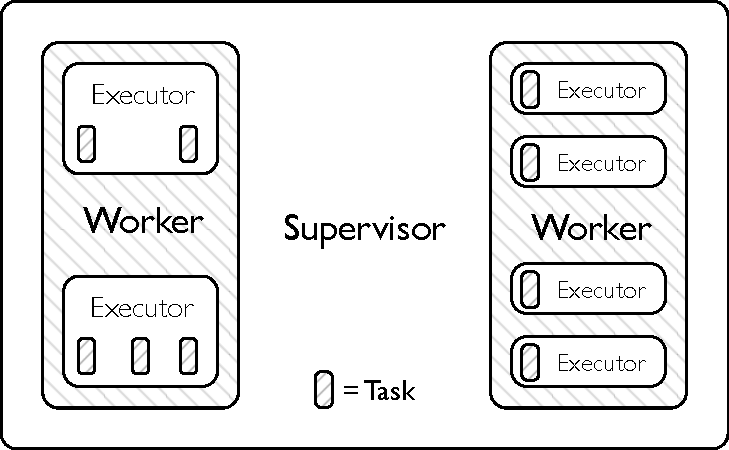
\includegraphics[width=0.95\linewidth]{pdf/distributed_worker.pdf}
  \caption{Worker node in Apache Storm.}
  \label{fig:comparison1}
\end{subfigure}\begin{subfigure}{.5\textwidth}
  \centering
  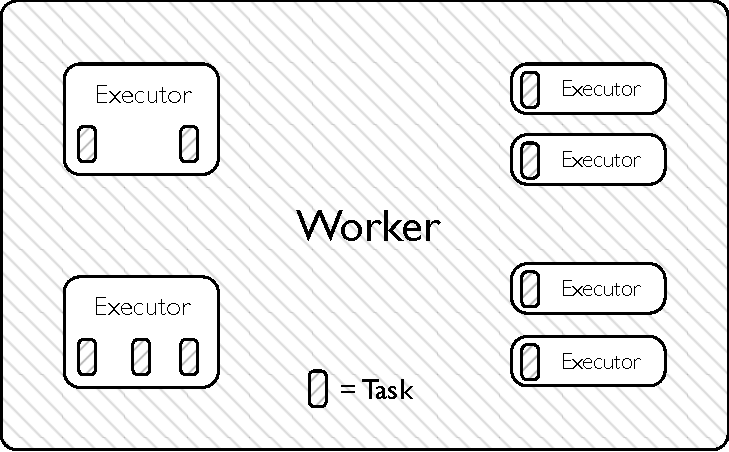
\includegraphics[width=0.95\linewidth]{pdf/local_worker.pdf}
  \caption{Worker node equivalent in Storm-MC.}
  \label{fig:comparison2}
\end{subfigure}
\caption{Comparison of a worker in Storm and Storm-MC}
\label{fig:comparison}
\end{figure}

The role of the worker wrapper is to launch executors and provide them with a shared context through which they can communicate. This is done with a map of Disruptor queues which the executors use as receive queues they pick tuples from.

Moreover, the worker wrapper contains a map of components and streams. This map specifies which bolts subscribe to a stream component produces. Executors use this map to figure out who they should send tuples to.

Additionally, the worker wrapper has a timer which components can use to get tick tuples at regular intervals. As mentioned before, bolts can use tick tuples to trigger events at regular intervals. For example, one might want to sort a window of tuples based on some criteria every five minutes.

Finally, a worker contains a configurable-size thread pool \texttt{ExecutorService}. Storm-MC executors can use this service via the topology context to launch background tasks on a shared thread pool.

\subsection{Removing State}

Storm-MC is completely stateless. The cluster state that was managed by Zookeeper in Apache Storm was completely stripped away. In Storm workers use the Zookeeper cluster state to communicate with Nimbus and vice versa. For example, when Nimbus creates topology assignments it informs workers via the cluster state. In Storm-MC, we adopted a more functional approach where worker is just a function invoked by the Nimbus part of the source code.

While this is not something that is visible to a user of Storm-MC, it required a great effort as all the code that used Zookeeper had to be refactored.

\subsection{Removing Serialisation}

Similarly to removing the Zookeeper state, great amount of work was put into removing the dependency of Storm-MC on Apache Thrift. This was mostly done to reduce code bloat and remove an unnecessary dependency since there is no serialisation required in a multi-core environment. Moreover, code generated by Thrift does not use standard Java camelCase naming conventions but instead uses underscore\_case. For example, Thrift generates method names such as \\ \texttt{get\_component\_common}.

This required refactoring all the data types generated automatically by Thrift. This not only reduced the size of the codebase significantly but also made the code more readable and self-documenting than the code generated by Thrift.

\section{Implementation Details}
\label{sec:implementation}

Most of the implementation was ported over from Storm-MC with adjustments where necessary. The problem with porting software is that there is a lot of functionality that needs to be changed but the changes required are usually not substantial. This section outlines details of Storm-MC implementation.

\subsection{Topology Submission}

Topologies are built using an instance of the \texttt{TopologyBuilder} class which uses the builder pattern - same as in Apache Storm. While the basis  of this class was reused from Storm, the internals had to be refactored so they work with data types used by Storm-MC. Once a topology is built it is submitted to an instance of \texttt{LocalCluster} class. This class is used in Storm for emulating the cluster on a local machine. Storm-MC adapted the class for backwards compatibility. This way, code created for Storm needs minimal adaptation to work on Storm-MC. A topology is submitted for execution via the \texttt{submitTopology} method which takes three arguments: the name of the topology, a Java Map with configuration, and a topology built by \texttt{TopologyBuilder}.

Users can submit a configuration file written in YAML. This is done by setting a JVM property called \texttt{storm.conf.file}. This file can for example define the capacity of the Disruptor queues, what waiting strategy should the components employ when there are no tuples to pick up, and what hooks they want executed every time a tuple is processed. Furthermore, users can define their own topology validator by implementing the \texttt{ITopologyValidator} interface.

\subsection{Tuple Processing}

\begin{figure}[!htb]
	\centering
	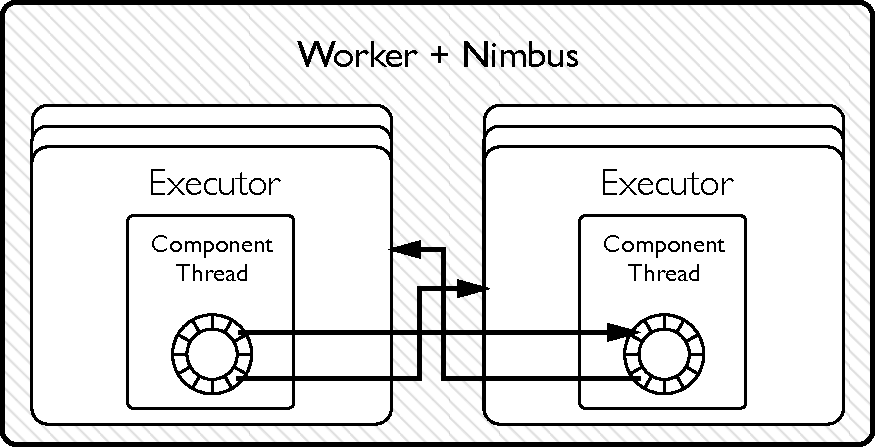
\includegraphics[scale=0.7]{pdf/worker_inside_mc.pdf}
	\caption{Tuple processing in Storm-MC.}
	\label{fig:worker_inside_mc}
\end{figure}

The implementation of tuple processing in Storm-MC is depicted in Figure \ref{fig:worker_inside_mc}. As can be seen from the figure, the queues used for remote message sending present in Storm were stripped away and there is only one Disruptor queue for every executor. Once an executor is done processing a tuple it puts it directly on the receive queue of its downstream bolts.

In Apache Storm, every executor runs two threads, one for tuple processing and one for tuple sending. In Storm-MC, however, there is only one thread per executor. Hence, the number of queues a tuple needs to pass through in a component is lowered as compared to Apache Storm.

Tuple processing in Storm-MC is a variant of multiple producer single consumer problem. In general, multiple producer single consumer problems are hard to optimise since there needs to be some form of synchronisation between multiple producers trying to produce an entry at the same time. In Disruptor queues this is implemented using the atomic Compare-and-Swap (CAS) operation. This operation ensures that even if multiple threads attempt to modify a variable only one of them succeeds and all threads involved are able to tell whether it was them that succeeded. Hence, one thread will succeed at claiming the next entry of a Disruptor queue and others will have to retry.

Alternatively, locks can be used used to synchronise access but lock-free queues using CAS are considered to be more efficient than locks because they do not require a kernel context switch \cite{Thompson_Farley_Barker_Gee_Stewart_2011}. However, even with CAS a processor must lock its instruction pipeline to ensure atomicity and employ a memory barrier to make the changes visible to other threads.

We investigated other data structures besides Disruptor queues that could be used for tuple exchange in Storm-MC but Disruptor queues are considered state of the art in low-latency parallel systems. This is one area that Apache Storm did really well and we were not able to further optimise.

Other options we considered were \texttt{ArrayBlockingQueue} and \texttt{LinkedBlockingQueue} both of which are in the Java standard library. However, the Disruptor shows superior throughput and latency compared to these options as shown in \citep{DisruptorWiki}.

\subsubsection{Waiting Strategies}

There are four different waiting strategies an executor can employ while waiting for a tuple to become available:

\begin{description}
	\item[BlockingWaitStrategy] \hfill \\
	This strategy uses a lock and a condition variable. The thread waits on the condition variable and is signalled once a new tuple becomes available. This strategy wastes the minimum number of CPU cycles when an executor is waiting.
	\item[SleepingWaitStrategy] \hfill \\
	This strategy initially spins for hundred iterations, then uses \texttt{Thread.yield()}, and finally uses \texttt{LockSupport.parkNanos(1L)} to sleep. Thus after quiet periods this strategy might introduce latency spikes.
	\item[YieldingWaitStrategy] \hfill \\
	This strategy initially spins for hundred iterations and then uses \texttt{Thread.yield()}. This strategy is a good compromise between CPU utilisation and great performance.
	\item[BusySpinWaitStrategy] \hfill \\
	In this strategy the thread is in a so-called tight loop, where it checks whether a new entry is available and only breaks out of the loop if there is a new entry. This strategy has the best performance but works well only if the number of CPU cores is higher than the number of active threads since it maximises CPU utilisation.
\end{description}

The default strategy used in Storm-MC is \texttt{BlockingWaitStrategy} but users can change the strategy in the configuration file.

\subsubsection{Tuple Pools}

Once a component wants to send a new tuple to its downstream components it needs to initialise a Java Tuple object. Here, we saw room for improvement since this might need to be done at very high rates, possibly million times per second.

Hence, a tuple pool was implemented where executors could place tuples after they were done with them so the tuples could be reused by other executors. However, access to this pool also had to be synchronised and hence accessing the pool introduced higher latency than simply initialising new tuples. Moreover, Java garbage collector actually does a good job of re-claiming unused memory and thus the idea of using a tuple pool was abandoned.

This problem could potentially be circumvented by using different constructs to achieve tuple passing but backwards compatibility with programs written for Apache Storm was deemed more important than the potential gain in performance.

\subsection{Executors}

The implementation of an executor processing a tuple is as follows:

\begin{enumerate}
	\item The executor repeatedly tries to pick a tuple from its Disruptor queue. If there are no tuples to be picked up it employs a waiting strategy between trials.
	\item Once it picks up a tuple, it processes it as per the component it represents.
	\item If it emits a new tuple it attempts to send it downstream by repeatedly trying to claim an entry of the downstream ring buffer.
	\item Once it successfully claims an entry it proceeds back to step 1.
\end{enumerate}

\section{Differences between Apache Storm and Storm-MC}
\label{sec:differences}

The codebase of Apache Storm is fairly large - 54,985 lines of code as reported by \texttt{cloc} \citep{Cloc}. Thus we had to prioritise features that were ported over to Storm-MC. Table \ref{table:features} presents a list of Storm features and shows which were ported over to Storm-MC and which were not.

\begin{table}[h!]
\centering
\small
\begin{tabular}{@{}lcc@{}}
    \textbf{Feature} & \textbf{Apache Storm} & \textbf{Storm-MC} \\ \toprule
    Multi-language Topologies & \cmark & \cmark \\
    Hooks & \cmark & \cmark \\
    Metrics & \cmark & \cmark \\
    Tick Tuples & \cmark & \cmark \\
    Multiple Topologies & \cmark & \xmark \\
    Topology Scheduling & \cmark & \xmark \\
	Trident API & \cmark & \xmark \\
    Built-in Metrics & \cmark & \xmark \\
    Nimbus as a Server & \cmark & \xmark \\
\end{tabular}
\caption{Feature comparison of Apache Storm and Storm-MC.}
\label{table:features}
\end{table}

A feature that we deemed very important is support for multi-language topologies. Thus, Storm-MC allows you to define components in other languages such as Python or Ruby and connect them into a Java topology. An example of a component defined in Python can be seen in Listing \ref{listing:wordcount_split_py}.

Storm-MC has support for task hooks just like Storm. Task hooks allow you to capture a number of events and execute custom code when the event occurs at a registered component. Hooks are created by subclassing \texttt{BaseTaskHook}. They can, for example, be used to update a web server with the latest performance metrics.

Additionally, Storm-MC has support for topology metrics. This way, components can record metrics such as number of tuples processed or a count of event occurrences. These metrics can then be automatically consumed by a bolt that subclasses the \texttt{MetricsConsumerBolt} class.

As mentioned before, Storm-MC supports tick tuples which can be used  to trigger component-local events at regular intervals.

Unlike Storm executing on a cluster, Storm-MC does not support running multiple topologies at the same time. However, to do that one only needs to run the topology in a separate process. This is because unlike when executing on the cluster different topologies do not need to share any state and it is more natural to execute them as separate processes. This design decision has the added benefit of each process having its own part of main memory thus reducing cache conflicts as shown in \citep{Chandra:2005:PIC:1042442.1043432} and providing higher security by not having different topologies share memory space.

Storm-MC does not support topology scheduling. Since within one process there is always only one topology running at a time and the hardware configuration of the machine does not change, the parallelism is clearly defined by the number of executors per component specified in the topology configuration.

One way to implement scheduling could be to pin threads to specific cores. Unfortunately, Java does not provide support for CPU affinity; the assignments are handled automatically by the JVM. Potentially, this could be achieved by using C or C++, both of which support CPU affinity, but this was not implemented in Storm-MC.

Apache Storm supports an alternative high-level API called Trident which then gets converted into spouts and bolts by the Storm library. Trident was omitted from Storm-MC but it would be possible to implement it on top of the current API.

Moreover, Apache Storm collects JVM metrics with a bolt called \texttt{SystemBolt}. This bolt is added automatically to all Storm topologies. This bolt is not included in Storm-MC topologies automatically but users can choose to add this bolt on their own.

Finally, Nimbus in Apache Storm performs as a server that clients can send topologies to for execution. In Storm-MC, we opted for a different design as outlined in previous sections. The interaction with the Nimbus service is usually through a shell script with a path to a JAR file of the topology and the main class to execute. This shell script was ported over to Storm-MC but instead of communicating with a service it spawns a new separate process that executes the topology.

\clearpage{}

\clearpage{}\clearpage{}

\clearpage{}\chapter{Evaluation}

This chapter evaluates Storm-MC. We describe the metrics used to evaluate performance of Storm-MC (\ref{sec:metrics}), list the configuration used for benchmarking (\ref{sec:system_conf}), compare Storm-MC to Apache Storm executing in local mode on a set of different topologies (\ref{sec:performance}), and finally talk about challenges encountered while designing Storm-MC (\ref{sec:challenges}).

\section{Evaluation Metrics}
\label{sec:metrics}

The system was evaluated on the following metrics:

\begin{description}
	\item[Throughput] \hfill \\
	The number of tuples processed by every component of the topology in the given time is recorded.
	\item[CPU Utilisation] \hfill \\
	The CPU utilisation is recorded every second throughout program execution and the average is computed.
	\item[Resident Memory Size] \hfill \\
	The resident size of main memory is recorded every second throughout program execution and the average is computed.
\end{description}

\section{System Configuration}
\label{sec:system_conf}

\subsection{Software Setup}

All performance benchmarks were ran using the following software packages:

\begin{itemize}
	\item Apache Storm version 0.9.2 \footnote{\url{https://github.com/mrknmc/storm/releases/v0.9.2-fix}}
	\item Storm-MC version 0.1.6 \footnote{\url{https://github.com/mrknmc/storm-mc/releases/0.1.6}}
	\item A fork of IBM Storm Email Benchmarks version 0.1.12 \footnote{\url{https://github.com/mrknmc/benchmarks/releases/0.1.12}}
	\item Storm-benchmark version 0.1.0 \footnote{\url{https://github.com/manuzhang/storm-benchmark}}
\end{itemize}

The Apache Storm source code had to be adapted to include a workaround for a deadlock bug present in version 0.9.2. This bug caused a topology to exit with threads left in Zombie state under certain conditions. This prevented Storm from logging the benchmark metrics after execution. Hence a workaround was added so the results were logged.

Version 0.1.6 is the latest version of Storm-MC as of this moment. The first release was version 0.1.0 which was production-ready but since then there were 6 minor versions fixing bugs as they were discovered during testing.

IBM open sourced a suite of benchmarks which they used to compare Apache Storm to their real-time stream system IBM Infosphere Streams \citep{InfoSphereStreams}. These benchmarks were adapted and used to benchmark Storm-MC against Apache Storm. The current version is 0.1.12.

Finally, a number of spout and bolt components were used from the storm-benchmark project which Apache Storm developers use to benchmark Storm.

Since Storm-MC reuses package names from Apache Storm, the same benchmark is directly executable by both libraries. This saved a lot of time and furthermore there is no need to maintain two benchmarks suites. An example topology submission to Storm-MC and Apache Storm, respectively would look as follows:

\begin{minted}{bash}
java -Dstorm.home=storm-mc -cp storm-multicore-0.1.6.jar
    ...
    -Dstorm.jar=storm-email-benchmark.jar
    com.ibm.streamsx.storm.email.benchmark.FileReadWordCount wordcount
java -Dstorm.home=apache-storm -cp storm-core-0.9.2-incubating.jar
    ...
    -Dstorm.jar=storm-email-benchmark.jar
    com.ibm.streamsx.storm.email.benchmark.FileReadWordCount wordcount
\end{minted}

In this example the Storm home directory was set, the corresponding library was added to the Java classpath, the JAR file containing the benchmark was submitted, and the main class and topology name were specified.

\subsection{Hardware Setup}

The machine used for benchmarking is the Informatics Student Compute server (\texttt{student.compute.inf.ed.ac.uk}). The server has the following hardware components:

\begin{description}
	\item[Processor: Intel\textsuperscript{\textregistered} Xeon\textsuperscript{\textregistered} E5-2690 v2 @ 3.00 GHz] \hfill \\
	The machine has two sockets with the same processor each. The processor has 10 physical cores with Hyper-Threading Technology which means it can handle up to 20 threads in parallel. Thus with two sockets, there is potential to execute up to 40 threads in parallel.
	\item[Main Memory] \hfill \\
	The machine has 378 GB of main memory. Since data stream processing uses windows to store only up to a certain amount of memory this was more than enough to conduct the benchmarks.
\end{description}

\subsection{Storm Configuration}

As mentioned before, when submitting a topology the programmer needs to submit a configuration file as well. To ensure that the performance difference between Apache Storm and Storm-MC was not caused by different configuration, the default configuration file from Storm 0.9.2 was used to benchmark both projects. Most notably, the size of the ring buffer used by executors \\ (\texttt{topology.executor.receive.buffer.size}) was set to 1024 and the wait strategy employed by executors when there are no tuples to pick up \\ (\texttt{topology.disruptor.wait.strategy}) was set to \texttt{BlockingWaitStrategy}.

\section{Results}
\label{sec:performance}

To assess performance of Storm-MC, 3 different benchmarks were executed, each with a different focus. The benchmarks were executed for a constant period of time - five minutes - after which the system was killed and metrics were collected. To avoid any performance differences caused by varying amounts of heap memory required by the tested systems, the programs were run with the following flag: \texttt{-Xmx10240M}. This flag sets the maximum amount of heap memory used by the JVM to 10 GB which was more than enough for all benchmarks.

The parallelism of components was varied from one to six and average CPU utilisation and resident memory size were recorded by the Unix \texttt{top} program \citep{UnixTop}. Maximum CPU utilisation with 40 threads is 4,000\%. Resident memory size is the amount of non-swapped physical memory a task has used. This metric can be deceiving as it depends on how OS manages memory but it is the only fairly reliable memory metric reported by \texttt{top} that can be used for Java programs. We only employ this metric to show proportional difference in memory usage between Storm and Storm-MC.

\subsection{WordCount Topology}

The first topology tested for performance is a variant of the aforementioned WordCount topology. This topology has a spout \texttt{FileReadSpout} generating random sentences, which sends messages to a \texttt{SplitSentenceBolt} bolt which splits the sentences on whitespace and sends individual words to a \texttt{CountBolt} which counts word frequencies. Recall, that this topology is shown graphically in Figure \ref{fig:wordcount_topology}. Since the components do not store any data in memory or make any I/O calls this topology is mostly CPU-bound.

The number of tuples processed by each component in Storm-MC and Apache Storm is shown in tables \ref{table:storm_mc_wordcount} and \ref{table:storm_wordcount}, respectively. As can be seen from the tables, not only was CPU utilisation in Storm-MC lower, Storm-MC often processed more than twice as many tuples per component than Apache Storm.  The number of tuples processed by \texttt{CountBolt}, the last component of the topology, is also show in Figure \ref{fig:countbolt-plot}. Since this topology is serial, the number of tuples processed by \texttt{CountBolt} is a good indicator of total throughput.

\begin{table}[!htb]
\begin{adjustwidth}{-0.5in}{-0.5in}
\centering
\small
\begin{tabular}{@{}rccccl@{}}
    \textbf{Parallelism} & \textbf{FileReadSpout} & \textbf{SplitSentenceBolt} & \textbf{CountBolt} & \textbf{CPU Utilisation} & \textbf{Resident Size} \\ \toprule
    1 & {25,767,502} & {25,767,502} & {225,815,174} & {217.9\%} & {690.8M} \\
    2 & {34,403,678} & {34,403,127} & {301,493,247} & {414.6\%} & {759.1M} \\
    3 & {45,731,188} & {45,732,988} & {400,767,999} & {611.5\%} & {798.4M} \\
    4 & {52,285,327} & {52,283,540} & {458,187,555} & {805.5\%} & {804.1M} \\
	5 & {55,326,941} & {55,325,167} & {484,844,652} & {998.7\%} & {806.0M} \\
	6 & {56,747,319} & {56,744,629} & {497,285,149} & {1,195.3\%} & {824.8M} \\
	10 & {40,341,798} & {40,336,962} & {353,490,567} & {1,967.4\%} & {2.7G} \\
\end{tabular}
\caption{Storm-MC: Tuples processed per component in WordCount Topology.}
\label{table:storm_mc_wordcount}
\end{adjustwidth}
\end{table}

\begin{table}[!htb]
\begin{adjustwidth}{-0.5in}{-0.5in}
\centering
\small
\begin{tabular}{@{}rccccl@{}}
    \textbf{Parallelism} & \textbf{FileReadSpout} & \textbf{SplitSentenceBolt} & \textbf{CountBolt} & \textbf{CPU Utilisation} & \textbf{Resident Size} \\ \toprule
    1 & {12,583,377} & {12,579,132} & {110,233,966} & {294.5\%} & {2.2G} \\
    2 & {16,800,475} & {16,796,695} & {147,194,709} & {481.7\%} & {2.8G} \\
    3 & {22,120,695} & {22,107,696} & {193,735,106} & {687.1\%} & {2.6G} \\
    4 & {20,720,637} & {20,711,756} & {181,500,586} & {895.3\%} & {2.6G} \\
	5 & {17,177,688} & {17,164,209} & {150,412,037} & {1,129.3\%} & {2.5G} \\
	6 & {17,402,418} & {17,388,691} & {152,374,303} & {1,342.1\%} & {2.3G} \\
	10 & {12,229,523} & {12,211,100} & {107,002,632} & {2,136.7\%} & {2.8G} \\
\end{tabular}
\caption{Apache Storm: Tuples processed per component in WordCount Topology.}
\label{table:storm_wordcount}
\end{adjustwidth}
\end{table}

\begin{knitrout}
\definecolor{shadecolor}{rgb}{0.969, 0.969, 0.969}\color{fgcolor}\begin{figure}[!htb]

{\centering 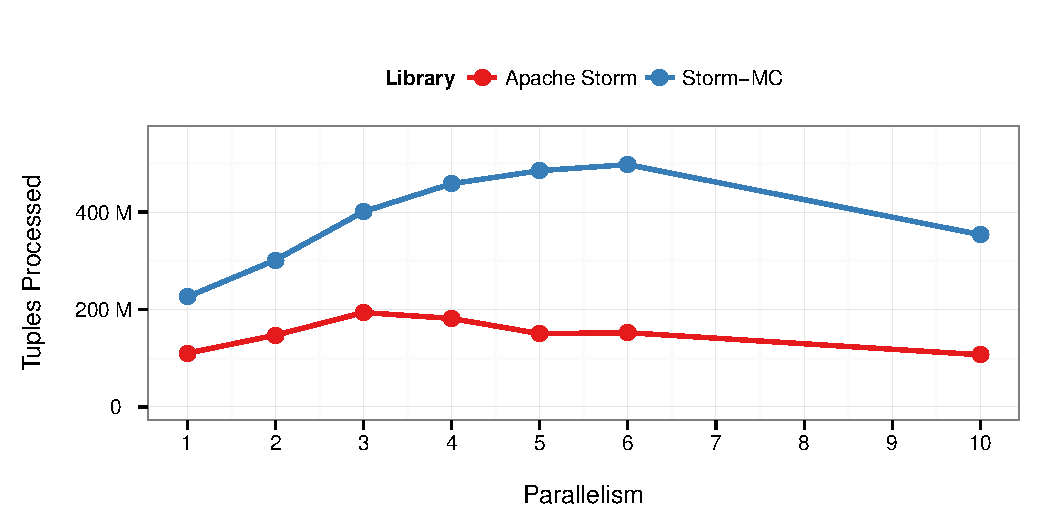
\includegraphics[width=\maxwidth]{figure/countbolt-plot-1} 

}

\caption[Tuples processed by CountBolt in Storm-MC and Apache Storm]{Tuples processed by CountBolt in Storm-MC and Apache Storm}\label{fig:countbolt-plot}
\end{figure}


\end{knitrout}

Furthermore, it can be seen that after the parallelism is increased beyond three the throughput of Apache Storm tails off and starts going down. This can be attributed to the number of threads ran by Apache Storm. For Storm-MC this tailing off occurs with parallelism of six where the overhead of multiple producers possibly trying to publish to the same queue becomes apparent. Moreover, with parallelism set to 6, Storm-MC executes with 20 threads which is close to the number of physical cores of the machine. However, it should be noted that even with parallelism equal to 10, Storm-MC still processes more than three times as many tuples as Storm.

\begin{knitrout}
\definecolor{shadecolor}{rgb}{0.969, 0.969, 0.969}\color{fgcolor}\begin{figure}[!htb]

{\centering 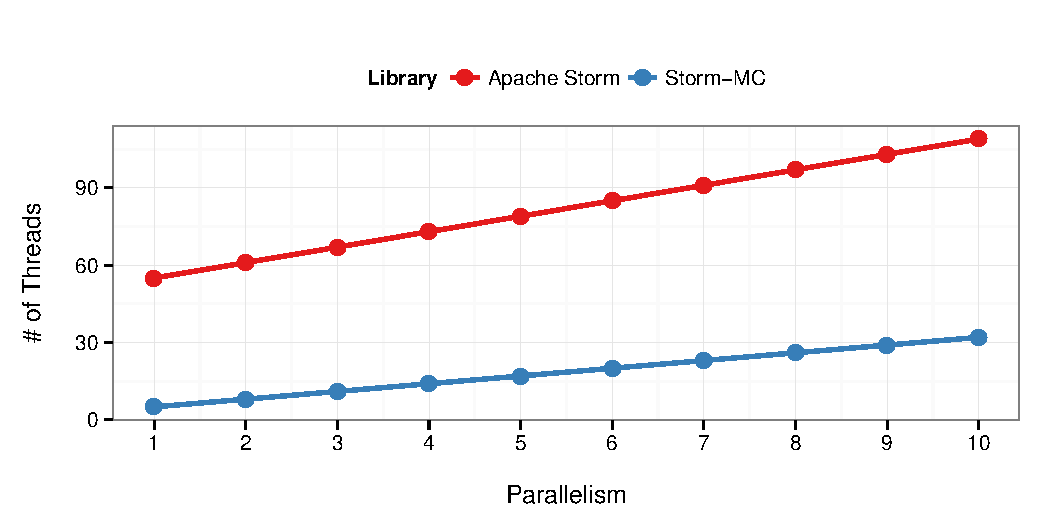
\includegraphics[width=\maxwidth]{figure/threads-plot-1} 

}

\caption[Number of threads used by Storm and Storm-MC]{Number of threads used by Storm and Storm-MC}\label{fig:threads-plot}
\end{figure}


\end{knitrout}

The number of threads required to execute a topology is a linear function of the parallelism for both Storm and Storm-MC. However, as shown in Figure \ref{fig:threads-plot}, the number of threads required by Storm increases more rapidly than Storm-MC. For example, with parallelism set to 10, Storm creates 109 threads whereas Storm-MC creates only 32. More formally, the number of threads required by both systems can be expressed as:

\begin{figure}[!htb]
\begin{eqnarray*}
	49 \ + \ 2 \times \sum\limits_{c}^{components} parallelism(c) && \text{ for Apache Storm.} \\
	2 \ + \ \sum\limits_{c}^{components} parallelism(c) && \text{ for Storm-MC.}
\end{eqnarray*}
\caption{Number of threads used by Storm and Storm-MC.}
\end{figure}

\textbf{N.B.}\@\xspace: This is a general formula that applies to all topologies, not just WordCount.

Of note, the resident size used by Storm-MC is also less than half of the resident size used by Storm for cases with parallelism less than 10.

\subsection{Enron Topology}

Next, Enron topology from the IBM benchmarks was tested for performance. In this topology, serialised emails from the Enron email dataset are read from a file by a \texttt{ReadEmailsDecompressSpout} spout. They are then deserialised by \texttt{AvroDeserializeBolt} bolt, filtered by \texttt{NewFilterBolt} bolt, modified by \texttt{ModifyBolt} bolt, and finally metrics are recorded by a \texttt{NewMetricsBolt} bolt. Additionally, every instance of the \texttt{NewMetricsBolt} bolt sends its local average email throughput to a global (excluded from the parallelism setting) \texttt{GlobalMetricsBolt} bolt every four seconds. This bolt then records the global average email throughput. Figure \ref{fig:enron_topology} shows this topology graphically.

\begin{figure}[!htb]
\begin{adjustwidth}{-0.5in}{-0.5in}
	\centering
	
\includegraphics[scale=0.475]{pdf/enron_topology.pdf}
	\caption{Enron topology.}
	\label{fig:enron_topology}
\end{adjustwidth}
\end{figure}

Similarly to the WordCount topology, this topology is serial in nature. However, whereas the spout in  WordCount topology keeps a small number of sentences in memory, the Enron topology has a spout that produces tuples by reading from a file. Thus, this benchmark is mostly I/O-bound. The average email throughput in Storm-MC and Apache Storm is shown in tables \ref{table:storm_mc_enron} and \ref{table:storm_enron}, respectively. 

\begin{table}[!htb]
\begin{adjustwidth}{-0.5in}{-0.5in}
\centering
\small
\begin{tabular}{@{}rccl@{}}
    \textbf{Parallelism} & \textbf{Emails Processed} & \textbf{CPU Utilisation} & \textbf{Resident Size} \\ \toprule
    1 & {3,285,742} & {297.7\%} & {806.8M} \\
    2 & {6,696,612} & {482.1\%} & {756.1M} \\
    3 & {8,493,772} & {729.5\%} & {341.4M} \\
    4 & {11,102,969} & {1036.9\%} & {326.0M} \\
    5 & {12,630,475} & {1311.0\%} & {260.8M} \\
    6 & {14,082,501} & {1590.3\%} & {334.0M} \\
\end{tabular}
\caption{Storm-MC: Email Throughput in Enron Topology.}
\label{table:storm_mc_enron}
\end{adjustwidth}
\end{table}

\begin{table}[!htb]
\begin{adjustwidth}{-0.5in}{-0.5in}
\centering
\small
\begin{tabular}{@{}rccl@{}}
    \textbf{Parallelism} & \textbf{Emails Processed} & \textbf{CPU Utilisation} & \textbf{Resident Size} \\ \toprule
    1 & {2,943,709} & {406.6\%} & {1.94G} \\
    2 & {4,832,874} & {945.1\%} & {2.93G} \\
    3 & {5,623,028} & {1,427.4\%} & {3.32G} \\
    4 & {6,238,395} & {1,891.2\%} & {3.56G} \\
    5 & {6,105,155} & {2167.4\%} & {3.65G} \\
    6 & {7,242,298} & {2388.6\%} & {4.09G} \\
\end{tabular}
\caption{Apache Storm: Email Throughput in Enron Topology.}
\label{table:storm_enron}
\end{adjustwidth}
\end{table}

\begin{knitrout}
\definecolor{shadecolor}{rgb}{0.969, 0.969, 0.969}\color{fgcolor}\begin{figure}[!htb]

{\centering 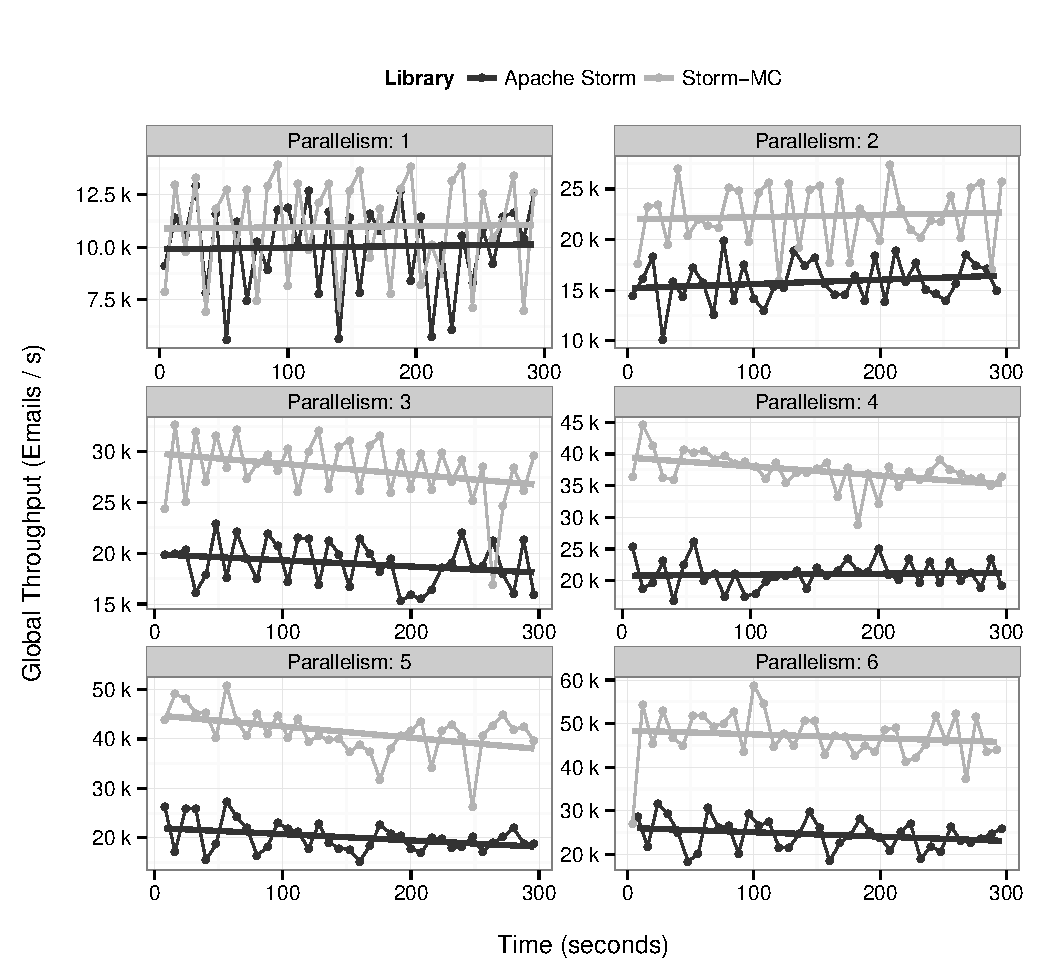
\includegraphics[width=\maxwidth]{figure/enron-plot-1} 

}

\caption[Global Email Throughput over time]{Global Email Throughput over time. Standard error shown in light grey.}\label{fig:enron-plot}
\end{figure}


\end{knitrout}

As can be seen from the tables, the difference in throughput in Enron Topology is less staggering than in WordCount. This is due to the fact that the throughput is limited by the file reads of the spout. However, as the parallelism increases the improvement in throughput of Storm-MC becomes more apparent as shown in Figure \ref{fig:enron-plot}. This figure also shows that the throughput is fairly volatile. This is due to the fact that the file is loaded into main memory in chunks and hence the throughput drops when the spout is trying to read from a file in between the loads. As before, the resident size used by Storm-MC is significantly lower than that of Storm.

\subsection{RollingSort Topology}

The RollingSort topology was ported over from the aforementioned storm-benchmark project. This topology only includes one spout sending tuples to one bolt. The \texttt{RandomMessageSpout} spout produces hundred character-long strings of random digits from zero to eight. The \texttt{SortBolt} bolt then stores a rolling window of hundred of such messages and sorts them every 10 seconds. The graphic representation of this topology can be seen in Figure \ref{fig:rolling_topology}.

\begin{figure}[!htb]
	\centering
	
\includegraphics[scale=0.475]{pdf/rolling_topology.pdf}
	\caption{RollingSort topology.}
	\label{fig:rolling_topology}
\end{figure}

This benchmark is considered to be memory-bound: the bolt stores a window of tuples in memory and performs a non-linear time sort. The results of running this benchmark on Storm-MC and Apache Storm can be seen in tables \ref{table:storm_mc_rolling} and \ref{table:storm_rolling}, respectively.

\begin{table}[!htb]
\begin{adjustwidth}{-0.5in}{-0.5in}
\centering
\small
\begin{tabular}{@{}rccccl@{}}
    \textbf{Parallelism} & \textbf{RandomMessageSpout} & \textbf{SortBolt} & \textbf{CPU Utilisation} & \textbf{Memory Usage} \\ \toprule
    1 & {249,143,444} & {249,142,400} & {186.2\%} & {504.3M} \\
    2 & {444,261,351} & {444,259,400} & {352.0\%} & {401.7M} \\
    3 & {350,861,061} & {350,859,800} & {514.7\%} & {382.9M} \\
    4 & {412,429,850} & {412,428,600} & {675.2\%} & {314.2M} \\
    5 & {470,813,184} & {470,811,300} & {835.8\%} & {423.2M} \\
    6 & {498,957,255} & {498,954,600} & {989.6\%} & {235.1M} \\
    7 & {519,744,352} & {519,741,700} & {1,149.0\%} & {637.9M} \\
    8 & {532,285,376} & {532,283,800} & {1,302.9\%} & {618.1M} \\
    9 & {501,519,539} & {501,517,700} & {1,430.4\%} & {579.4M} \\
    10 & {555,468,830} & {555,467,000} & {1,651.6\%} & {564.7M} \\ 
\end{tabular}
\caption{Storm-MC: Tuples processed per component in RollingSort Topology.}
\label{table:storm_mc_rolling}
\end{adjustwidth}
\end{table}

\begin{table}[!htb]
\begin{adjustwidth}{-0.5in}{-0.5in}
\centering
\small
\begin{tabular}{@{}rccccl@{}}
    \textbf{Parallelism} & \textbf{RandomMessageSpout} & \textbf{SortBolt} & \textbf{CPU Utilisation} & \textbf{Memory Usage} \\ \toprule
    1 & {173,906,935} & {173,900,300} & {267.3\%} & {3.0G} \\
    2 & {226,583,924} & {226,579,200} & {468.3\%} & {3.0G} \\
    3 & {310,949,455} & {310,943,000} & {634.6\%} & {2.9G} \\
    4 & {362,675,336} & {362,663,600} & {815.2\%} & {2.8G} \\
    5 & {409,470,032} & {409,462,100} & {969.4\%} & {2.7G} \\
    6 & {435,471,042} & {435,459,600} & {1,139.6\%} & {2.6G} \\
    7 & {395,386,336} & {395,309,900} & {1,327.7\%} & {2.6G} \\
    8 & {366,680,402} & {366,553,300} & {1,509.1\%} & {2.7G} \\
    9 & {359,091,633} & {358,942,200} & {1,689.5\%} & {2.7G} \\
    10 & {313,912,451} & {313,811,300} & {1,889.5\%} & {2.7G} \\
\end{tabular}
\caption{Apache Storm: Tuples processed per component in RollingSort Topology.}
\label{table:storm_rolling}
\end{adjustwidth}
\end{table}

While Storm-MC still outperforms Apache Storm, the difference in performance is marginal. This is due to the fact that the topology only has two components and the application is mostly memory bound. Storm-MC provides speed improvements for topologies that are mostly CPU-bound and have several components working serially such as WordCount. Furthermore, Storm-MC beats Storm significantly when the parallelism is high, as in previous topologies.

\section{Challenges}
\label{sec:challenges}

In this section we are going to discuss challenges we encountered while porting Apache Storm to multi-core machines.

\begin{description}
	\item[Unfamiliarity with Clojure] \hfill \\
	One of the main challenges while working on this project was learning a new programming language - Clojure. Since most of the implementation of Apache Storm is written in Clojure, this language had to be studied and its concepts well understood for us to be able to write code that worked with the existing codebase. By the end of the project writing Clojure became as simple as writing Java.
	\item[Lack of Documentation] \hfill \\
	Even though Apache Storm is a popular project documentation is available only for the high level concepts used within Storm. The implementation details are often obscured away in hard to understand functions. Since the documentation is lacking our knowledge of Storm had to be obtained by reading the source code of an initially unfamiliar language. By the end of the project the Storm-MC code became well documented and we might attempt back-porting to Apache Storm.
\end{description}

\clearpage{}

\clearpage{}\chapter{Conclusion}

This final chapter concludes with a summary of contributions of this project (\ref{sec:contribs}) and discusses future work that could stem from this project (\ref{sec:future_work}).

\section{Summary of Contributions}
\label{sec:contribs}

The primary contribution of this project is Storm-MC - a library aimed at data stream processing applications. The benefits of using Storm-MC are twofold:

\begin{itemize}
	\item It offers the same easy-to-use API as Apache Storm.
	\item It is tailored to multi-core environments.
\end{itemize}

Since Storm-MC uses the same API as Apache Storm, applications written with Storm in mind can be ported to use Storm-MC with minimum amount of effort. Thus if an application requires parallelism satisfiable by a single multi-core machine, it can be executed on one machine instead of a cluster.

Moreover, the Storm API allows programmers to create data stream processing applications on multi-core with an unprecedented ease. All of this comes with the superior performance Storm-MC offers compared to running Apache Storm in local mode, as shown in Section \ref{sec:performance}.

\section{Future Work}
\label{sec:future_work}

Storm-MC could be improved in a number of ways:

\begin{description}
	\item[Storm-MC as a Server] \hfill \\
	Storm-MC could be updated to enable it to run as a server. This could have several benefits such as being able to execute multiple topologies at the same time with a thin wrapper that could control their execution just like with Apache Storm. This was not implemented as we assumed most of the time users are executing only one topology per machine.
	\item[Higher Level Abstractions] \hfill \\
	Defining components of a Storm-MC topology is fairly simple. Programmers only need to define how components are connected, how they process tuples, and what tuples they emit. However, this could be taken even further with the user only specifying high-level functions and the Storm-MC library figuring out how to distribute the work. In Apache Storm this is implemented in Trident which was not ported as part of this project.
	\item[Automatic Parallelism] \hfill \\
	Sometimes when configuring a topology it may be difficult to predict the rate at which spouts are going to produce tuples. If the rate is underestimated consumers could be lagging behind producers. On the other hand, if the rate is overestimated consumers could be idle, not doing any useful work. Thus it might be advantageous to have an automatic parallelism setting which could add or remove consumers based on the current tuple rate.
	
	It may seem that this would be trivial to implement with a pool of threads representing one component. However, there are several problems that need to be considered. For example, fields grouping guarantees that tuples with the same field values go to the same executor. Changing the parallelism at runtime breaks this guarantee.
	
	Alternatively each executor could use a pool of threads. This comes with its own set of problems: the executor object would have to provide synchronised access to the pool which would only increase latency. Hence, implementing automatic parallelism was out of the scope of this project.
	\item[Performance Comparison with Distributed Storm] \hfill \\
	The benchmarks in this report compared Storm-MC to Apache Storm running in local mode. It would be interesting to see how Storm-MC compares to Apache Storm running on a cluster. One could compare the number of nodes to the number of CPUs required to execute a topology. This could provide 
\end{description}
\clearpage{}

\pagenumbering{Roman}

\begin{appendices}
	\clearpage{}\chapter{Listings}
\label{ch:listings}

\begin{listing}[!htb]
\inputminted[frame=lines,linenos]{java}{code/RandomSentenceSpout.java}
\caption[RandomSentenceSpout.java]{RandomSentenceSpout.java: Definition of a spout that emits a randomly chosen sentence from a predefined collection of sentences.}
\label{listing:wordcount_spout}
\end{listing}

\begin{listing}[!htb]
\inputminted[frame=lines,linenos]{java}{code/SplitSentence.java}
\caption[SplitSentence.java]{SplitSentence.java: Definition of a bolt that executes a Python script.}
\label{listing:wordcount_split}
\end{listing}

\begin{listing}[!htb]
\inputminted[frame=lines,linenos]{python}{code/splitsentence.py}
\caption[splitsentence.py]{splitsentence.py: Definition of a bolt that splits sentences on whitespace in Python.}
\label{listing:wordcount_split_py}
\end{listing}

\begin{listing}[!htb]
\inputminted[frame=lines,linenos]{java}{code/WordCount.java}
\caption[WordCount.java]{WordCount.java: Definition of a bolt that counts word frequencies.}
\label{listing:wordcount_count}
\end{listing}

\clearpage{}
\end{appendices}

\printbibliography

\end{document}
